\documentclass[12pt]{extarticle}
\usepackage{tempora}
\usepackage[T1, T2A]{fontenc}
\usepackage[utf8]{inputenc}
\usepackage[english, ukrainian]{babel}
\usepackage{geometry}
\usepackage{graphicx}
\usepackage{multirow}
\usepackage{multicol}
\usepackage{float}
\graphicspath{{/home/artem/Pictures}}
\geometry
{
    a4paper,
    left=30mm,
    top=15mm,
    right=20mm,
    bottom=15mm,
}

\begin{document}
\begin{titlepage}
    \begin{center}
        \textbf{\normalsize{\MakeUppercase{
            Міністерство Освіти і науки України
            Національний університет "Львівська політехніка"
        }}}

        \begin{flushright}
        \textbf{ІКНІ}\\
        Кафедра \textbf{ПЗ}
        \end{flushright}
        \vspace{15mm}

        \includegraphics[width=0.4\textwidth]{lpnu_logo.png}

        \vspace*{\fill}

        \textbf{\normalsize{\MakeUppercase{Звіт}}}
            
        До лабораторної роботи №3

        \textbf{на тему:} “ Метод швидкого сортування”

        \textbf{з дисципліни:} "Алгоритми і структури даних”
            
        \vspace*{\fill}

        \begin{flushright}

            \textbf{Лектор:}\\
            доцент кафедри ПЗ\\
            Коротєєва Т. О.\\
            \vspace{12pt}

            \textbf{Виконав:}\\
            студент групи ПЗ-24\\
            Губик А. С.\\
            \vspace{12pt}

            \textbf{Прийняв:}\\
            асистент кафедри ПЗ\\
            Вишневський О. К.\\
        \vspace{12pt}
        \end{flushright}

        Львів -- 2023
            
            
    \end{center}
\end{titlepage}

\subsection*{Тема роботи} 
Метод швидкого сортування.



\subsection*{Мета роботи}  Вивчити алгоритм швидкого сортування. 
Здійснити програмну реалізацію алгоритму швидкого сортування. 
Дослідити швидкодію алгоритму швидкого сортування.

\subsection*{Індивідуальне завдання}
Задано одномірний масив дійсних чисел. Виключити з нього моду (елемент, який повторюється найчастіше). Отриманий масив посортувати в порядку зростання.

\subsection*{Теоретичні відомості}
Швидке сортування (англійською «Quick Sort») — алгоритм сортування, добре відомий, як алгоритм розроблений Чарльзом Хоаром, який не потребує додаткової пам’яті і виконує у середньому $O(n log(n))$ операцій. Оскільки алгоритм використовує дуже прості цикли і операції, він працює швидше інших алгоритмів, що мають таку ж асимптотичну оцінку складності.

В основі алгоритму лежить принцип «розділяй та володарюй» (англійською «Divide and Conquer»). Ідея алгоритму полягає в переставлянні елементів масиву таким чином, щоб його можна було розділити на дві частини і кожний елемент з першої частини був не більший за будь-який елемент з другої. Впорядкування кожної з частин відбувається рекурсивно. Алгоритм швидкого сортування може бути реалізований як на масиві, так і на двобічному списку.

Швидке сортування є алгоритмом на основі порівнянь, і не є стабільним.

Алгоритм швидкого сортування було розроблено Чарльзом Хоаром у 1962 році під час роботи у маленькій британській компанії Elliott Brothers.

В класичному варіанті, запропонованому Хоаром, з масиву обирався один елемент, і весь масив розбивався на дві частини по принципу: в першій частині — ті що не більші даного елементу, в другій частині — ті що не менші даного елемента.

Час роботи алгоритму сортування залежить від збалансованості, що характеризує розбиття. Збалансованість, у свою чергу залежить від того, який елемент обрано як опорний (відносно якого елемента виконується розбиття). Якщо розбиття збалансоване, то асимптотично алгоритм працює так само швидко як і алгоритм сортування злиттям. 

Найгірше розбиття. Найгірша поведінка має місце у тому випадку, коли процедура, що виконує розбиття, породжує одну підзадачу з (n – 1) елементом, а другу — з 0 елементами. Нехай таке незбалансоване розбиття виникає при кожному рекурсивному виклику. Для самого розбиття потрібен час $\theta(n)$. Тоді рекурентне співвідношення для часу роботи, можна записати наступним чином:$ T(n) = T(n – 1) + T(0) + \theta(n) = T(n ­– 1) + \theta(n). $
Найкраще розбиття. В найкращому випадку процедура поділу ділить задачу на дві підзадачі, розмір кожної з яких не перевищує (n / 2). Час роботи, описується нерівністю: $T(n) <= 2T(n / 2) + \theta(n). Тоді: T(n) = O(n log(n))$ — асимптотично найкращий час.
      Математичне очікування часу роботи алгоритму на всіх можливих вхідних масивах є $O(n log(n))$, тобто середній випадок ближчий до найкращого.

В середньому алгоритм працює дуже швидко, але на практиці, не всі можливі вхідні масиви мають однакову імовірність. Тоді, шляхом додання рандомізації вдається отримати середній час роботи в будь-якому випадку. В рандомізованому алгоритмі, при кожному розбитті в якості опорного обирається випадковий елемент.


\subsection*{Покроковий опис} 

\begin{enumerate}

\item \textbf{Функція:} Знаходимо елемент який найчастіше зустрічається і видаляємо його.

\item \textbf{Вибір елемента-опори:} Виберіть елемент-опору з масиву. Вибір елемента-опори може вплинути на продуктивність алгоритму. Зазвичай вибирають перший, останній, середній або випадковий елемент з масиву.
\item \textbf{Розділення:} Перегрупуйте елементи
 масиву так, щоб елементи менше за елемент-опору опинилися зліва від 
 нього, а елементи більше за елемент-опор опинилися справа. 
 Сам елемент-опор опиняється на своєму остаточному відсортованому місці. 
 Цей процес часто називають розділенням.

Ініціалізуйте два вказівника: один на початку масиву, інший на його кінці.
Переміщуйте вказівник зліва вправо, доки не знайдете елемент, який більший або рівний елементу-опору.
Переміщуйте вказівник справа вліво, доки не знайдете елемент, який менший або рівний елементу-опору.
Поміняйте місцями елементи, на які вказують ці вказівники.
Повторюйте ці кроки, доки вказівник зліва не стане більшим або рівним вказівнику справа. Елемент-опор тепер опинився на своєму остаточному відсортованому місці, і всі елементи ліворуч менше його, а всі елементи праворуч більше нього.
\item \textbf{Рекурсія:} Рекурсивно застосовуйте алгоритм 
Quick Sort до підмасивів ліворуч і праворуч від елемента-опори. 
Цей процес триває до тих пір, поки підмасиви не містять лише по 
одному елементу, який вже є відсортованим.
\item \textbf{Об'єднання:} Після того, як всі рекурсивні виклики повернуться, вихідний масив вже відсортований. Підмасиви об'єднуються, і отримуємо остаточно відсортований масив.

\end{enumerate}

\subsection*{Вихідний код}

{\fontfamily{pcr}\selectfont

\begin{verbatim}
    #include <iostream>
    #include <vector>
    #include <cstdlib>
    #include <ctime>
    #include <algorithm>
    #include <chrono>
    
    // Custom quick sort function
    void quickSort(std::vector<float>& arr, int left, int right) {
        if (left < right) {
            float pivot = arr[left];
            int i = left, j = right;
    
            while (i < j) {
                while (i < j && arr[j] >= pivot) {
                    j--;
                }
                if (i < j) {
                    arr[i++] = arr[j];
                }
    
                while (i < j && arr[i] <= pivot) {
                    i++;
                }
                if (i < j) {
                    arr[j--] = arr[i];
                }
            }
    
            arr[i] = pivot;
    
            // Print the vector at each iteration
            std::cout << "Iteration " << (left - right) / 2 << ": ";
            for (const float& num : arr) {
                std::cout << num << " ";
            }
            std::cout << std::endl;
    
            quickSort(arr, left, i - 1);
            quickSort(arr, i + 1, right);
        }
    }
    
    int main() {
        // Seed the random number generator
        std::srand(static_cast<unsigned>(std::time(nullptr)));
    
        // Get the size of the vector from the user
        int vectorSize;
        std::cout << "Enter the size of the vector: ";
        std::cin >> vectorSize;
    
        // Generate a vector of random float numbers
        std::vector<float> numbers;
        for (int i = 0; i < vectorSize; i++) {
            float randomFloat = static_cast<float>(std::rand()) / static_cast<float>(RAND_MAX);
            numbers.push_back(randomFloat);
        }
    
        std::cout << "Unsorted Vector:" << std::endl;
        for (const float& num : numbers) {
            std::cout << num << " ";
        }
        std::cout << std::endl;
        // Measure sorting time
        auto startTime = std::chrono::high_resolution_clock::now();
    
        // Sort the vector using custom quick sort
        quickSort(numbers, 0, numbers.size() - 1);
    
        auto endTime = std::chrono::high_resolution_clock::now();
        auto duration = std::chrono::duration_cast<std::chrono::nanoseconds>(endTime - startTime);
    
        float median;
        if (vectorSize % 2 == 0) {
            median = (numbers[vectorSize / 2 - 1] + numbers[vectorSize / 2]) / 2.0f;
        } else {
            median = numbers[vectorSize / 2];
        }
    
        numbers.erase(std::remove(numbers.begin(), numbers.end(), median), numbers.end());
    
        // Print the sorted vector
        std::cout << "Sorted Vector:" << std::endl;
        for (const float& num : numbers) {
            std::cout << num << " ";
        }
        std::cout << std::endl;
    
        std::cout << "Sorting time: " << duration.count() << " nanoseconds" << std::endl;
    
        return 0;
    }
    
\end{verbatim}
}
\vspace{12pt}
\begin{figure}[H]
    \centering
    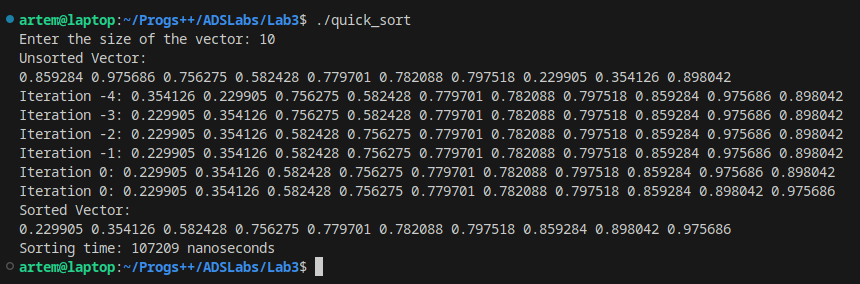
\includegraphics[width=0.90\textwidth]{Screenshot_20231017_234955.png}
    \caption{}
\end{figure}
\subsection*{Висновок} 
Основна ідея в Quick Sort полягає в розділенні масиву, що
 дозволяє ефективно перегрупувати елементи навколо елемента-опори, 
 зменшуючи кількість елементів, які потребують сортування в кожному
  рекурсивному виклику. Quick Sort має середню та найкращу складність
   часу O(n log n), що робить його одним з найшвидших алгоритмів 
   сортування на практиці.
\end{document}
